% This must be in the first 5 lines to tell arXiv to use pdfLaTeX, which is strongly recommended.
\pdfoutput=1
% In particular, the hyperref package requires pdfLaTeX in order to break URLs across lines.

\documentclass[11pt]{article}

\usepackage[usenames,dvipsnames]{xcolor}
% Remove the "review" option to generate the final version.
% \usepackage[review]{acl}
\usepackage[]{acl}

% Standard package includes
\usepackage{times}
\usepackage{latexsym}

% For proper rendering and hyphenation of words containing Latin characters (including in bib files)
\usepackage[T1]{fontenc}
% For Vietnamese characters
% \usepackage[T5]{fontenc}
% See https://www.latex-project.org/help/documentation/encguide.pdf for other character sets

% This assumes your files are encoded as UTF8
\usepackage[utf8]{inputenc}

% This is not strictly necessary, and may be commented out,
% but it will improve the layout of the manuscript,
% and will typically save some space.
\usepackage{microtype}

% If the title and author information does not fit in the area allocated, uncomment the following
%
%\setlength\titlebox{<dim>}
%
% and set <dim> to something 5cm or larger.

\title{CLAfICLe: Cross Lingual Adaptation for In-Context Learning}

% Author information can be set in various styles:
% For several authors from the same institution:
% \author{Author 1 \and ... \and Author n \\
%         Address line \\ ... \\ Address line}
% if the names do not fit well on one line use
%         Author 1 \\ {\bf Author 2} \\ ... \\ {\bf Author n} \\
% For authors from different institutions:
% \author{Author 1 \\ Address line \\  ... \\ Address line
%         \And  ... \And
%         Author n \\ Address line \\ ... \\ Address line}
% To start a seperate ``row'' of authors use \AND, as in
% \author{Author 1 \\ Address line \\  ... \\ Address line
%         \AND
%         Author 2 \\ Address line \\ ... \\ Address line \And
%         Author 3 \\ Address line \\ ... \\ Address line}

\author{Giulio Starace \\
  University of Amsterdam / Amsterdam, The Netherlands \\
  \texttt{giulio.starace@gmail.com} \\}

% user settings
\usepackage{graphicx} % for images
\usepackage{subcaption} % for subfigures
\graphicspath{{../figures/}}
\usepackage[export]{adjustbox}
\usepackage{geometry}
\usepackage{booktabs}


\begin{document}
\maketitle
\begin{abstract}
	This document is a supplement to the general instructions for *ACL authors. It contains instructions for using the \LaTeX{} style files for ACL conferences.
	The document itself conforms to its own specifications, and is therefore an example of what your manuscript should look like.
	These instructions should be used both for papers submitted for review and for final versions of accepted papers.
\end{abstract}

\section{Introduction}

contributions
\begin{itemize}
	\item successfully apply WECHSEL to GPT2 Large, release the checkpoints which did not exist
	\item More complete evaluation of WECHSEL in the GPT2 setting
	\item propose method for preserving FT when performing cross-lingual adaptation
	\item formalize concept of vessel adapters with targeted distillation, a form of post-hoc disentanglement
\end{itemize}

\section{Related Work}

\section{Method}\label{sec:method}
\begin{figure*}[ht]
	\subcaptionbox{\label{fig:sandwich}}
	{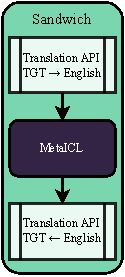
\includegraphics{sandwich.pdf}}
	\hfill
	\subcaptionbox{\label{fig:metaicl-gewechselt}}
	{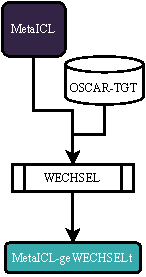
\includegraphics{metaicl-gewechselt.pdf}}
	\hfill
	\subcaptionbox{}
	{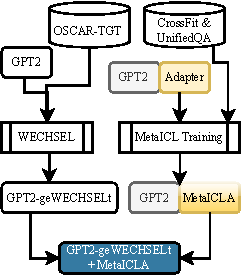
\includegraphics{gpt2-gewechselt+metaicla.pdf}}
	\hfill
	\subcaptionbox{}
	{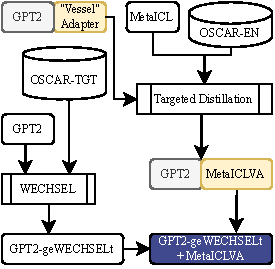
\includegraphics{gpt2-gewechselt+metaiclva.pdf}}
	\caption{Overview of each of the models evaluated in one of the two TGT
		languages (French or German). The baseline
		\textcolor[HTML]{79d6ae}{Sandwich} model (\subref{fig:sandwich}) sandwiches
		\textcolor[HTML]{332345}{MetaICL} \citep{min_metaicl_2022} (which we
		separately evaluate only in English) between two complementary translation
		API calls. \textcolor[HTML]{38AAAC}{MetaICL-geWECHSELt}
		(\subref{fig:metaicl-gewechselt}) is the result of applying WECHSEL
		\citep{minixhofer_wechsel_2022} to MetaICL.
		\textcolor[HTML]{357aa2}{GPT2-geWECHSELt+MetaICLA} combines
		\textcolor{Dandelion}{MetaICLA}, an adapter trained on the MetaICL dataset
		and objective, with a TGT-language GPT2 base obtained via WECHSEL.
		\textcolor[HTML]{40498e}{GPT2-geWECHSELt+MetaICLVA} does the same, except
		\textcolor{Dandelion}{MetaICLVA} is trained via targeted distillation with
		supervision provided by MetaICL. For more details, refer to section
		\ref{sec:method}.}
\end{figure*}

\section{Results and Discussion}
\begin{figure}[ht]
	\centering
	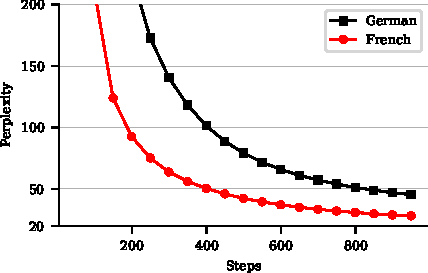
\includegraphics[width=0.9\linewidth]{gpt2-w_ppl.pdf}
	\caption{Perplexity on the held out set when performing the recommended CLM training after WECHSEL
		language-adaptation of GPT2. A step corresponds to an optimizer update. We evaluate every 50
		steps.}
	\label{fig:gpt2-w_ppl}
\end{figure}

Fig.\@ \ref{fig:gpt2-w_ppl} shows the performance of GPT2 after around 1k steps of training, evaluated
intrinsically in terms of perplexity. For both French and German, we see perplexity decrease to
sub-50 values, with the French model reaching a perplexity of $\approx$ 28. Both models are clearly
underfit, still monotonically decreasing by the end of the training. These observations are roughly
in-line with \citet{minixhofer_wechsel_2022}'s findings for smaller variants of GPT2, although we
train for much less time and hence are left with higher perplexities. While we believe our
preliminary results suggest WECHSEL scales well to larger models in terms of intrinsic evaluation,
future work may wish to investigate whether this holds for longer training times. The rest of our
work considers, among other questions, the robustness of WECHSEL via extrinsic evaluation on
downstream tasks performed by MetaICL.

\begin{figure*}
	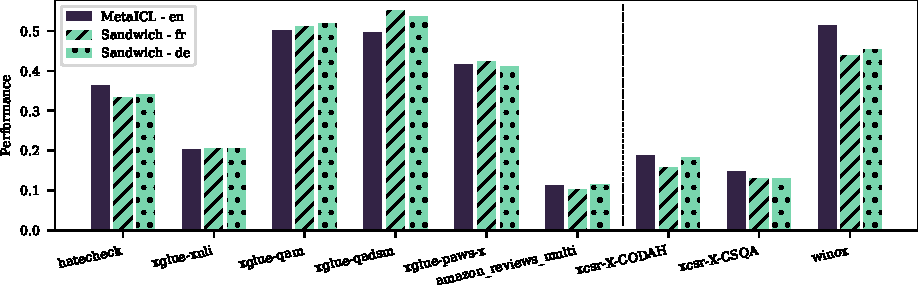
\includegraphics{baselines.pdf}
	\caption{Performance (max is 1) on a particular language dimension of our multi-task benchmark of
		our two baseline models, MetaICL and Sandwich. The dashed line separates whether a given task uses
		accuracy (left) or F1-score (right) as the performance metric.}
	\label{fig:baselines}
\end{figure*}

Fig.\@ \ref{fig:baselines} shows the performance on each dataset of our benchmark for the two baseline
models, MetaICL and Sandwich. As summarized in Table \ref{tab:results-summary}, Sandwich performs
roughly on-par with MetaICL on both target languages, respectively with scores of 0.317 and 0.322 in
French and German compared to MetaICL's score of 0.327 in English. We note generally low scores
across all tasks. This is particularly perplexing in the case of MetaICL, scoring around 0.1 points
less than with the evaluation ensemble used by \citet{min_metaicl_2022}, where the same checkpoint
was reported scoring 0.417 in the worst case (a 25 \% decrease). While similar values are reached in certain tasks in
our benchmark (e.g. most of XGLUE and WINO-X), it is unclear what the origin of this discrepancy is,
whether due to differences in evaluation implementation or difficulty of the tasks. Given that
\citet{min_metaicl_2022} simply report macro-averaged scores, it is impossible to verify the latter.
Nevertheless, our results suggest that Sandwich-like solutions may be satisfactory for transferring
performance from English to other languages given the surprisingly closeness of the scores. The
decision between using Sandwich or ``properly'' adapted models with the same capabilities then
becomes an economic one in terms of the cost of API calls (for the former) vs the cost of
inference plus training (for the latter).

\begin{figure*}[ht]
	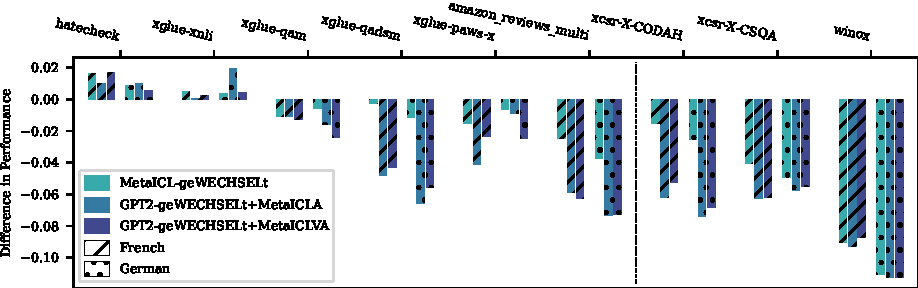
\includegraphics{results.pdf}
	\caption{Performance gap on our multi-task benchmark between each of the language-adapted models
		and the ``Sandwich'' baseline. Positive values indicate that the adapted models are
		outperforming the baseline, while negative values indicate the reverse. The dashed line
		separates whether a given task uses accuracy (left) or F1-score (right) as the performance
		metric.}
	\label{fig:results}
\end{figure*}

Fig.\@ \ref{fig:results} shows the difference in performance on each dataset of our benchmark between
the proposed models and Sandwich. In general, we observe that the proposed models underperform
across almost all tasks in both French and German, with the trends aligning at a task-level (e.g.
all models underperform on QAM, by roughly the same amount). As reported in Table
\ref{tab:results-summary}, the best of our proposed models is MetaICL-geWECHSELt, which
underperformed Sandwich by roughly 0.02-0.03 points. This undermines the motivation for the other
two models, which were designed to avoid catastrophic forgetting by separating language and ICL
capabilities via adapters. The results suggest that the tradeoff between catastrophic forgetting and
needing to train ICL-adapters leans in favour of the former in this compute regime. In this sense,
we can conclude that WECHSEL does not suffer tremendously due to catastrophic forgetting when
adapting fine-tuned causal language models such as the MetaICL variant of GPT2.

Future work should
\begin{itemize}
	\item todo
\end{itemize}



% Please add the following required packages to your document preamble:
% \usepackage{booktabs}
\begin{table}[ht]
	\centering
	\caption{Average performance (max is 1) across the datasets from our multi-task benchmark for the
		models considered in this work. We use ``W'' as a shorthand for ``geWECHSELt''. We report average
		difference in performance for each proposed alternative to Sandwich. Negative values indicate
		underperformance compared to Sandwich.}
	\label{tab:results-summary}
	\begin{tabular}{@{}rccc@{}}
		\toprule
		\multicolumn{1}{c}{} & en    & fr     & de                             \\ \midrule
		MetaICL              & 0.327 & -      & -                              \\
		Sandwich             & -     & 0.317  & 0.322                          \\ \midrule
		\multicolumn{4}{c}{\textit{Difference in Performance w.r.t. Sandwich}} \\
		MetaICL-W            & -     & -0.020 & -0.026                         \\
		GPT2-W+MetaICLA      & -     & -0.041 & -0.042                         \\
		GPT2-W+MetaICLVA     & -     & -0.036 & -0.045                         \\ \bottomrule
	\end{tabular}
\end{table}

\section{Conclusion}

\bibliography{anthology,custom}

\section{Appendices}

Use \verb|\appendix| before any appendix section to switch the section numbering over to letters. See Appendix~\ref{sec:appendix} for an example.

\appendix
\section{Example Appendix}
\label{sec:appendix}

This is an appendix.

\end{document}
